\chapter{MATERIALS AND METHODS}
\label{chap:Materials}

The research in this dissertation is about mobile robotic manipulators. As outlined in the literature review, the mobile manipulator can be controlled either jointly or as two separate systems: a mobile base and a robotic manipulator, the latter being a case in this dissertation. Thus, the research can be broadly divided into two parts, one tackling the navigation of mobile base and the other deals with the estimation of forces acting on the manipulator end-effector, since those forces are the key to successful completion of tasks in which the robot interacts with a human, other robot or anything in its environment. 

Mobile robot navigation can be described as a robot to the desired goal and avoiding both static and dynamic obstacles on the way. Since this complex behaviour consists of two simpler ones, the goal was to develop an approach to the mobile robot navigation in which these behaviours are developed separately, and outputs of the two are then fused to achieve the complex behaviour.

First, a neural network-based obstacle avoidance method was developed, as described in Section \ref{sec:MMAvoidance} \cite{Kruzic2020}, which is then used in the fusion scheme called \emph{mediation}, described in Section \ref{sec:MMMediation} \cite{Music2019}. Finally, an approach to manipulator end-effector force estimation based on deep neural networks is presented in Section \ref{sec:MMForceEstimation} \cite{Kruzic2020a}. In each section, a problem is formulated, and a method to solve the problem is given. The appropriate experiments were conducted to assess the viability and performance of the presented solutions to the problems in question.


\section{Neural network-based obstacle avoidance}
\label{sec:MMAvoidance}

\subsection{Problem formulation}

The goal of this part of the research was to develop a procedure to train and test an efficient neural network architecture for mobile robot obstacle avoidance while keeping human intervention as minimal as possible (i.e., self-supervised nature) \cite{Kruzic2020a}. The approach should provide numerous positive and negative examples (negative examples about the crashes) to the learning algorithm but should safely do that for the robot and its environment.  It should also enable the collection of large amounts of data with minimal effort and cost. To that end, it was decided to use 2D LiDAR instead of a camera for several reasons. First, although cameras can provide much more data than LiDAR, LiDAR provides sufficient data for obstacle avoidance. Second, however, it should be kept in mind that LiDAR sensing can fail in some instances (e.g., in the presence of glass surfaces or if the distance is below or above the sensing threshold). 

Furthermore, the LiDAR output is less complex than the video stream, making the neural network architecture simpler and shorter training time. This less complex nature of input data has an attractive side effect that real-world measurements are more similar to simulation-based ones than in the case of a video stream. Finally, mass-produced and low-cost LiDARs are on the horizon, making them a logical choice for one of the mobile robot's primary sensors for the future.

There are two fundamental reasons why simulation was chosen for conducting this research. The first one is that crashing a real robot into obstacles may damage both the robot and the environment. The other is that the usage of simulation makes possible the collection of large amounts of data with different crashing scenarios with minimal effort and negligible cost, yet achieving a high degree of similarity between data obtained in simulation compared to real-world data by using LiDAR sensor. An additional reason for using a simulation environment is that the whole approach (including neural networks) can be fine-tuned in simulation and deployed only when an acceptable level of performance is achieved (as was done in the research).

Differences between the simulated camera and LiDAR compared to the real-world camera and LiDAR data are illustrated in Figure \ref{fig:Fig01}. From the figure, it can be seen that differences exist between the simulation and real-world cases both for LiDAR and camera. However, due to different lighting conditions (which are difficult to reproduce in simulation) and the existence of textures and shadows, the image-based comparison produces more significant discrepancies than the LiDAR-based one. Please note that the same distance from the robot to obstacles was used in both scenarios. It should be noted that recently approach which uses simple graphics (i.e., not photorealistic) but with a substantial number of variations in light and texture (for better generalisation) have been investigated and good results reported \cite{Bousmalis2018}.

\begin{figure}
    \centering
    \subfloat[Camera image from simulation environment]{\includegraphics[width=0.45\textwidth]{slike/turkish/Fig01a.png}}
    \hfill
    \subfloat[Camera image from real robot]{\includegraphics[width=0.45\textwidth]{slike/turkish/Fig01c.png}}
    \vfill
    \subfloat[LiDAR data from simulation environment]{\includegraphics[width=0.45\textwidth]{slike/turkish/Fig01b.png}}
    \hfil
    \subfloat[LiDAR data from real robot]{\includegraphics[width=0.45\textwidth]{slike/turkish/Fig01d.png}}
    \caption{Differences between camera images and laser scans in simulation and on the real robot of the approximately same scene.}
    \label{fig:Fig01}
\end{figure}

Please note that, although simulation-based neural network training approaches do exist in the literature (as is already presented in Chapter \ref{chap:Literature}), they usually employ cameras (which provide RGB images), use complex convolutional neural networks for obstacle avoidance, do not collect both positive and negative examples, and do not do the neural network training process automatically. The focus of the research was thus to develop the approach that would enable collecting the right amount of data needed for training neural networks for obstacle avoidance in a self-supervised manner in simulation. Furthermore, it should also be answered if simulation-driven LiDAR data can be effectively used for training neural networks and seamlessly transferred to real-world applications and how do such neural networks perform in the real world compared to some common obstacle avoidance algorithms.

\subsection{Data collection and labelling}

Training data was generated and collected in Gazebo simulation environment \cite{Koenig2004} as follows. First, a simulation was automatically initialised, and various obstacles were randomly scattered within it, as is shown in Figure \ref{fig:Fig02}. The dimensions of the simulated environment were always kept the same (12.5 m $\times$ 12.5 m) but can be freely chosen/changed by the user. Then, the robot was spawned in its centre with random orientation and was given a constant linear velocity of 0.4 m/s. While the robot was in motion, LiDAR data were collected. The recording was carried out until the robot crashed into the obstacle or the perimeter wall.

\begin{figure}
    \centering
    \subfloat[Gazebo world and various obstacle shapes. Please note that obstacles had footprints of 0.5 m $\times$ 0.5 m for cubes, 4 m $\times$ 0.8 m for cuboids and 0.5 m $\times$ 0.5 m for cylinders.]{\includegraphics[width=0.9\textwidth]{slike/turkish/Fig02a.pdf}}
    \vfill
    \subfloat[Examples of different randomly generated Gazebo Worlds]{\includegraphics[width=0.9\columnwidth]{slike/turkish/Fig02b.pdf}}
    \caption{Gazebo simulation environment}
    \label{fig:Fig02}
\end{figure}

The laser range finder scans were timestamped, and the timestamp of the moment when the robot hits the obstacle was also recorded. Eventually, the preceding procedure is repeated many times (specified by the user) to obtain enough data for the neural networks to generalise appropriately. In our experiments, we obtained a total of 3,754 crash events (in 19 simulation worlds with different obstacle setups), which took about two workdays of real-time self-supervised execution (with no human intervention) on a computer with an Intel Core i3 6100 processor and 4 GB of RAM. The described data collection procedure resulted in 396,377 training samples (both positive and negative ones).

Before the training of the neural networks, the obtained data were preprocessed. First, failed LiDAR measurements were replaced with maximal possible range values. Failed measurements occurred when the obstacle was closer than the declared minimum sensor range (0.15 m) or farther away than the maximum (6 m). Obtained scan data was then divided into three overlapping groups, so each of the three networks was trained on a different dataset. The network for the forward motion used scans of 45$^{\circ}$ to both left and right of forward direction (90$^{\circ}$ in total), while the network for left and right motion used scans of 90$^{\circ}$ to the left and the right of the forward direction. This is graphically depicted in Figure \ref{fig:Fig03} (from the robot's viewpoint).

The last two seconds of the robot motion before the collision were treated as negative examples (this duration was always guaranteed since there were no obstacles in an appropriate diameter around the robot's initial position), but only for the network(s) representing the side of the robot on which the bumper was activated during the collision. In contrast, the other sides' network labels remained positive. If a particular measurement lasted longer than 4 s, the first 2 s were treated as positive examples while the remaining (middle) part of the data samples (excluding the last two seconds) was discarded and not used for training. Otherwise, all remaining data samples were treated as positive examples.

\begin{figure}
    \centering
    \includegraphics[width=0.75\textwidth]{slike/turkish/Fig03.pdf}
    \caption{LiDAR scans divided into three overlapping groups (left, forward, right)}
    \label{fig:Fig03}
\end{figure}

After initial labelling, all the labels are further examined, and those that are positive are converted to negative if there were some laser scan points closer than the predefined threshold. The relabelling procedure was conducted to prevent motion near the obstacles that did not result in a crash. An example of such a situation would be a robot moving parallel to the wall. The decision about if a label needed to be converted to negative was made based on two parameters: the number of laser scan points and the threshold. Both parameters varied during the study (using predefined values of 3, 5, and 7 for the points and 0.4 m, 0.6 m, 0.8 m and 1 m for thresholds. The procedure of how a label is classified using these numbers of points and thresholds is given in Figure \ref{fig:Threshold}. The label is negative if there are 3, 5 or 7 LiDAR points under the appropriate dashed line, depending on the chosen threshold value. 

\begin{figure}
    \centering
    \includegraphics[width=0.9\textwidth]{slike/thr.png}
    \caption{The classification of LiDAR scan points in the presence of a complex obstacle}
    \label{fig:Threshold}
\end{figure}

In such a way, 12 datasets were created to identify which pair of parameters (number of points, threshold) were optimal for the task. Then, neural networks were trained for each pair of values for the number of points and a threshold to identify which pair of these values performs best for the task \cite{Kruzic2018}. The intention was to keep neural networks trained with data from the dataset with parameters that were proved optimal and use them for further experimenting.

The whole labelling and neural networks training procedure is given as Algorithm \ref{Alg:Preprocess}.

\begin{algorithm}
\caption{Data preprocessing and neural networks training procedure}
\label{Alg:Preprocess}
\begin{algorithmic}
	\renewcommand{\algorithmicrequire}{\textbf{Input:}}
    \renewcommand{\algorithmicensure}{\textbf{Output:}}
    \REQUIRE LiDAR scan $S$
    \STATE Replace failed measurements in $S$ with max LiDAR range
    \STATE Forward: $S_F \gets S_{1:45} \cup S_{316:360}$
    \STATE Left: $S_L \gets S_{1:90}$
    \STATE Right: $S_R \gets S_{271:360}$
    \STATE Points: $P \gets \{3,5,7\}$
    \STATE Thresholds: $T \gets \{0.4, 0.6, 0.8, 1.0\}$
    \FOR {$p$ in points}
      \FOR {$t$ in thresholds}
          \STATE Label $S_F$, $S_L$, $S_R$ using $p$ and $t$
          \STATE Train $\mathrm{NN}_F^{(p,t)}$, $\mathrm{NN}_L^{(p,t)}$, $\mathrm{NN}_R^{(p,t)}$
      \ENDFOR
    \ENDFOR
    %\ENSURE $\mathrm{NN_F}$, $\mathrm{NN_L}$, $\mathrm{NN_R}$
    \ENSURE $\{\mathrm{NN}_F^{(p,t)}$, $\mathrm{NN}_L^{(p,t)}$, $\mathrm{NN}_R^{(p,t)} \mid p \in $ pts $\land~t \in$ thresholds $\}$
\end{algorithmic}
\end{algorithm}


\subsection{Neural networks training}

The neural network-based controller was designed to have three independent neural networks: left, forward, and right. Several network architectures were considered and trained using different hidden layers numbers (1 to 4), and different neurons per layer (20, 40, 60, 16 different network architectures per direction (left, right and forward) were trained, giving a total of 48 architectures, whose performance was analysed. Each network was trained as a multilayer perceptron, using MATLAB Deep Learning Toolbox, with scaled gradient descent as the optimiser and mean squared error (MSE) as the loss function (and performance metric). The performance of all trained networks was analysed on the validation set (the analysis is given in Section XYZ). Based on the analysis, the optimal architecture for the task is identified.

% Prebaciti u rezultate
%\begin{figure}
    %\centering
    %\includegraphics[width=0.8\textwidth]{slike/turkish/Fig04.pdf}
    %\caption{Performance analysis for different trained NN architectures based on MSE metric obtained on validation set}
    %\label{fig:Fig04}
%\end{figure}

%\begin{figure}
    %\centering
    %\includegraphics[width=\textwidth]{slike/turkish/Fig05.pdf}
    %\caption{Selected NN architecture used in the experiments}
    %\label{fig:Fig05}
%\end{figure}

Once the optimal architecture is identified, the neural network was trained with samples from randomly selected 75\%, 50\% and 25\% of data samples (297,283, 198,189 and 99,095 training samples, respectively) in order to approximately estimate the number of collisions needed for proper generalisation of neural networks. 

Based on the neural network outputs, velocity and angular velocity commands are computed using the policy in Algorithm \ref{Alg:Policy} as follows. Each neural network output was between 0 and 1, which is the probability that the space in the appropriate direction is obstacle-free. Alternatively, one may think of this as the output of 1 meaning \emph{``go in this direction''} and 0 meaning \emph{``do not go in this direction''}. Network outputs are post-processed to obtain linear ($v$) and angular ($\omega$) velocities for robot motion. If the forward direction probability ($P(F)$) was above a predefined threshold of 0.5 (which was determined experimentally), then the direction was computed as a proportion to a difference between probabilities of left and right directions ($P(L)$ and $P(R)$, respectively) being obstacle-free. If the forward direction probability were below the threshold, the robot would slow down to a low positive velocity and not stop to avoid local minima (also experimentally determined and explained in Section \ref{Sec:ResLabelling}) and rotate either to the left or right depending on which side is obstacle-free. Once forward-facing neural network probability increased above the threshold, it would speed up and continue as before. Thus, it can be concluded that linear velocity had two predefined levels, while the angular velocity could attain any value between -2 rad/s and 2 rad/s, and the value is computed using Equation \ref{eq:AngularVelocity}.

\begin{algorithm}
\caption{Obstacle avoidance policy used in testing}
\label{Alg:Policy}
\begin{algorithmic}
	\renewcommand{\algorithmicrequire}{\textbf{Input:}}
    \renewcommand{\algorithmicensure}{\textbf{Output:}}
    \REQUIRE Scans $S_F$, $S_L$, $S_R$, neural networks $\Theta_F$, $\Theta_L$, $\Theta_R$
    \STATE Forward probability: $P(F) = \Theta_F(S_F) \in [0,1]$
    \STATE Left probability: $P(L) = \Theta_L(S_L) \in [0,1]$
    \STATE Right probability: $P(R) = \Theta_R(S_R) \in [0,1]$
    \IF {$P(F)>0.6$}
    	\STATE $v=0.4$ m/s
        \STATE $\omega\propto P(L)-P(R)$
    \ELSE
    	\STATE $v=0.08$ m/s
        \IF {$P(L)>P(R)$}
        	\STATE $\omega\propto P(L)$
        \ELSE
        	\STATE $\omega\propto -P(R)$
        \ENDIF
    \ENDIF
    \ENSURE $(v,\omega)$
\end{algorithmic}
\end{algorithm}

\begin{gather}
    \label{eq:AngularVelocity}
    \omega = \begin{cases}
        \hphantom{-}2 \cdot P(L) & P(L) \geq P(R)\\
        -2 \cdot  P(R) & P(L) < P(R)
    \end{cases}\\
    P(L), P(R) \in [0,1] \nonumber
\end{gather}

\subsection{Experimental setup}

Several experiments were performed in order to assess the performance of the proposed approach. The first experiment was conducted to identify optimal parameters for data labelling. The obtained results are then used in other experiments, both in simulation and in the real world, to show that neural networks trained on simulation data can perform well without any retraining. %There were experiments conducted in simulation, as well as those conducted on a real-world robot.

\subsubsection{Labelling parameters experiments}
\label{Sec:MMLabelling}

An experiment was conducted to assess the performance of neural networks trained on simulation data and deployed on a real robot. The environment for testing the approach was a relatively narrow (2.16 m) corridor augmented with additional obstacles, as shown in Figure \ref{Fig:Hodnik}.

\begin{figure}
\centering
\includegraphics[width=0.9\textwidth]{slike/hodnik}
\caption{Testing environment}
\label{Fig:Hodnik}
\end{figure}

Each of 12 datasets was used for testing with five trials per dataset, resulting in 60 trials. The robot was left to roam in the course freely. There was no allocated time frame for task completion. However, there were four events in the case of which a trial terminated: completion of the course (i.e. going beyond the last obstacles on the course, see Figure \ref{Fig:LabellingTraj}), crash into obstacle or walls, stuck in a loop (i.e. repeating the same motions over and over) or stuck at local minimum (i.e. when moving forward is not possible, and when robot executes in-place rotation left and right interchangeably).

\subsubsection{Simulation experiments}

The first experiment was conducted in simulation in four random environments that were generated the same way as were those used for collecting training data and shown in Figure \ref{fig:Fig02}. There were five test runs in each of the environments (20 test runs in total). Each run began with the robot in the centre with a random orientation. It lasted until the robot crashed into the obstacle, or a maximum time limit of 10 minutes was reached.

The second simulation experiment was straightforward and was conducted in a small 5 m x 5 m environment with a single moving obstacle, as depicted in Figure \ref{fig:Fig07}. The robot was left for 10 minutes to roam around the environment. The experiment was run four times, each time with a different (but constant) obstacle velocity (0.1 m/s, 0.2 m/s, 0.4 m/s and 0.8 m/s; please note that in the Figure \ref{fig:Fig07}, the obstacle moved back and forth in the directions indicated by the arrows). 

\begin{figure}
    \centering
    \includegraphics[width=0.5\textwidth]{slike/turkish/Fig07.pdf}
    \caption{Simulation environment for testing robot behaviour in the presence of moving obstacle. Arrows indicate motion directions of the moving obstacle.}
    \label{fig:Fig07}
\end{figure}

\subsubsection{Real-world experiments}

Other experiments were conducted in the real world on a real robot using (heavily modified) Turtlebot 2 mobile robot (shown in Figure \ref{fig:Fig08}), with a LiDAR sensor mounted on-board. The 2D LiDAR used was Rplidar-A1M8, which has a resolution of 1 degree (i.e., gives 360 points per measurement cycle) and run with a 7 Hz rotation frequency. 

In the first real-world experiment, a U-shaped obstacle was used to test how well the neural network recovers from such a complex obstacle and a challenging situation. In contrast, in the second one, a narrow (only 2.16 m wide) corridor was augmented with additional obstacles making it more demanding for the obstacle avoidance algorithm. The experimental setup for this experiment is similar to the one described in Section \ref{Sec:MMLabelling}, but the dataset used for the training neural networks was preprocessed with the values identified in the mentioned experiment (described in Section \ref{Sec:ResLabelling}), and there were fewer obstacles (but the same corridor was used).

\begin{figure}
    \centering
    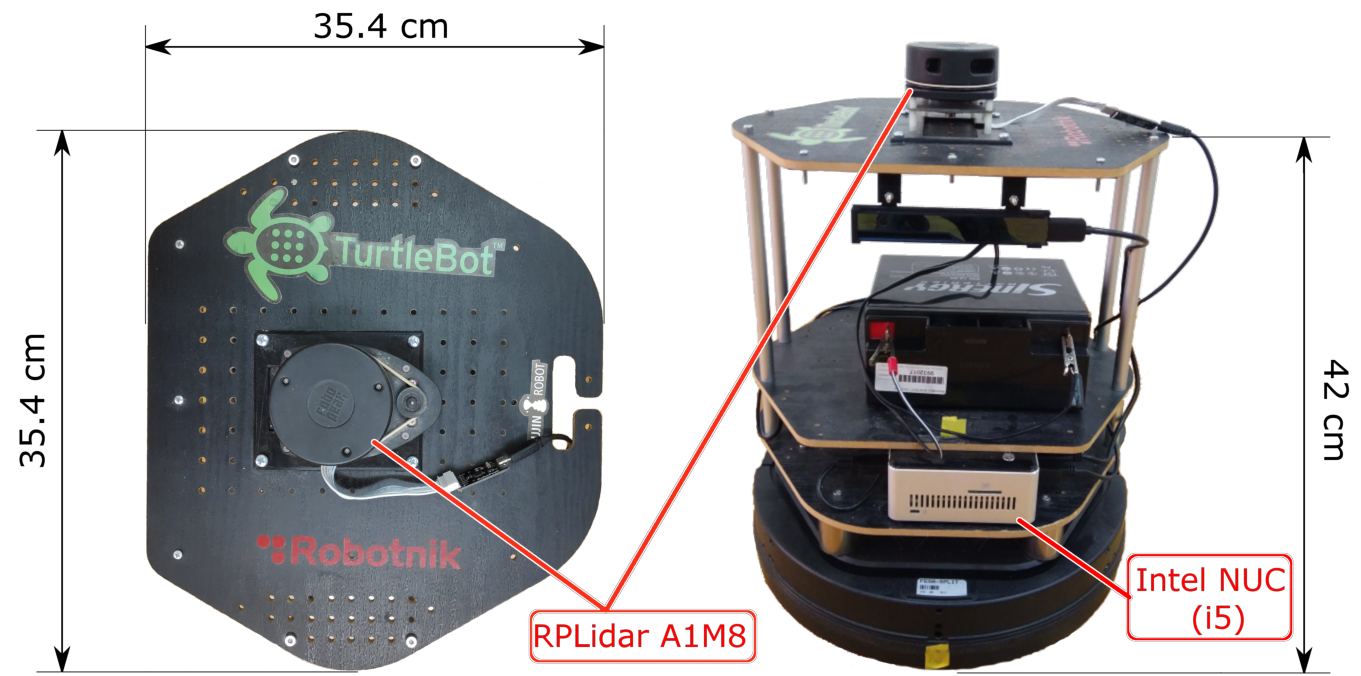
\includegraphics[width=0.9\textwidth]{slike/turkish/Fig08.pdf}
    \caption{Turtlebot 2 mobile robot, used in real-world experiments}
    \label{fig:Fig08}
\end{figure}

In the corridor test case (Figure \ref{fig:Fig10}), obstacles were placed in such a manner that it could be, with a high degree of certainty, assumed that the obstacle avoidance will fail (since free gaps at the last obstacle - rightmost one in Figure \ref{fig:Fig10c} - are well below the clearances used in training).

Afterwards, the proposed approach was compared to a more standard obstacle avoidance algorithm shipped with ROS (Robot Operating System) \cite{Quigley2009} navigation stack - Dynamic Window Approach (DWA) \cite{Fox1997}. The measurement setup was pretty simple, with the robot always starting from the same point in space and having to go to the point behind a simple rectangle-shaped obstacle that was not in the original map.

In the final real-world experiment, the robot was placed inside a complex, self-contained obstacle course (similar to the simulated environment) which is shown in Figure \ref{fig:Fig12}, and in which it freely ran for 20 minutes. The course also had dynamic obstacles (moving mobile robots Turtlebot 3 Burger and Waffle) with predefined trajectories. The number of collisions, the time between collisions as well as the distance between collisions were recorded. 

\begin{figure}
    \centering
    \subfloat[Ground plan of the complex obstacle course where the final experiment was conducted, with marked starting positions of test vehicle and moving obstacles. Dotted lines show predefined trajectories of moving obstacles (Turtlebot 3 mobile robots).]{\includegraphics[width=0.9\textwidth]{slike/turkish/Fig12a.pdf}}
    \vfill
    \subfloat[A snapshot of real-world testing environment]{\includegraphics[width=0.9\textwidth]{slike/turkish/Fig12b.pdf}}
    \caption{Real-world testing environment with static and dynamic obstacles}
    \label{fig:Fig12}
\end{figure}

\section{Mediated navigation}
\label{sec:MMMediation}

\subsection{Problem formulation}

From the literature review, it can be concluded that deploying state-of-the-art autonomous capabilities to a mobile robot usually entails developing complex neural network-based architectures and training them in an end-to-end fashion on large datasets (either in a simulation or in a real-world environment). Furthermore, if different behaviour is required, a new network needs to be developed or an existing one retrained (and new training data generated or recorded). 

It is desirable to develop an approach to mobile robot navigation that will allow existing control algorithms and combine them with artificial intelligence. In the field of control theory, there exist approaches by which complex robot behaviour is achieved by \emph{mediation} between two desired behaviours \cite{Vincenti2009}. Therefore, complex behaviours, such as navigation, can be divided into simpler ones. Thus, for each simple behaviour, another controller can be in charge. With this approach, it is possible to achieve that to perform slightly different tasks by the robot does not need to change the whole approach to the problem, but it is enough to change one of the controllers in charge of the behaviour we want to change, which saves time and achieves complex patterns of mobile robot behaviour. 

Implementing a mediator that would enable the fusion of control signals from several sources (including, but not limited to, neural networks) is proposed to avoid training new networks when the new behaviour is required. One possible function on which adaptive control in mobile robot navigation tasks could be based is collision probability \cite{Lunenburg2017} since obstacle avoidance usually has the highest priority in the navigation stack hierarchy. The mediation can be implemented in several forms, and one of them is based on fuzzy set theory \cite{Chen2017}. It is worth noting that several \emph{mediation engines} can be used in the process, as well as several decision functions based on which the mediator infers the final decision and thus adapts the robot behaviour \cite{Vincenti2009}.

Overview of the proposed adaptive fuzzy control scheme can be seen in Figure \ref{Fig:Blok} which shows that the approach uses two controllers (neural networks or any other type of controller) whose inputs are combined within fuzzy set theory based on the collision probability as the decision variable. The collision probability parameter is explained in more detail later on.

\begin{figure}
\centering
\includegraphics[width=0.95\columnwidth]{slike/blok.png}
\caption{The general control architecture of the proposed approach.} 
\label{Fig:Blok}
\end{figure}

In the proposed approach, one controller was used for reaching the goal position without regard to obstacles (navigation controller), while the other controller was used solely for obstacle avoidance without regard to the goal position. Furthermore, both controllers (in the case of neural networks) were trained using data obtained in the simulation, making the proposed approach safe and straightforward. 

The neural network-based obstacle avoidance controller that was used in this part of the research consisted of three neural networks (for left, right and forward) and is described in detail in Section \ref{sec:MMAvoidance} with Algorithm \ref{Alg:Policy} used to generate velocity commands as outputs of the controller. The velocity part of the command is always at one of two predefined levels (0.4 m/s and 0.08 m/s), and the angular velocity is given as

\begin{gather}
    \label{eq:AngularVelocity2}
    \omega_A = \begin{cases}
        \hphantom{-}2 \cdot P(L) & P(L) \geq P(R)\\
        -2 \cdot  P(R) & P(L) < P(R)
    \end{cases}\\
    P(L), P(R) \in [0,1] \nonumber
\end{gather}

Please note that the Equation \ref{eq:AngularVelocity2} is just rewritten version of the Equation \ref{eq:AngularVelocity} to accommodate the notation used in Figure \ref{Fig:Blok}.

In the case of the development of a neural network for navigation, the following procedure was taken. First, a single user was asked to drive a Turtlebot 2 mobile robot in the Gazebo simulation from a random starting point to a random goal within a 25 m $\times$ 25 m environment without any obstacles. The driver was instructed to give equal importance to the accuracy and the speed of driving. During the driving, the robot position was recorded, thus making it possible to calculate the distance from the goal. This procedure was repeated 700 times, giving a total of 380,541 training examples. After that, the recorded data was used to train a simple neural network (for regression) with four layers of 30 neurons each. This architecture was (as was the case for neural network-based obstacle avoidance) determined experimentally as the one with good enough performance. As an input, the network was given the error in position (i.e., distance to the goal) and orientation (i.e., the difference between the current and the final orientation). In addition, the network was given both the linear and angular velocities recorded during the trials as the targets. Also, these were used as its output during testing. After the training, the approach was tested successfully in environments without obstacles, both in simulation and real life. 

Additionally, in cases when a simple Proportional (P)-type controller was used, its output was such that it kept the linear velocity ($v_N$) constant till the goal was reached. In contrast, angular velocity ($\omega_N$) changed depending on the difference between the current and desired position (both in the odometer frame of reference). In this manner, both the simple and more complex (neural network-based) cases of navigation controllers were taken into account.

The outputs from the neural network-based obstacle controller and from the navigation controller (being any of the types used in the research) were then fed to the fuzzy mediation block, where the consensus decision was made (based on $\zeta$ value) and adapted linear ($v$) and angular ($\omega$) velocities were generated.

\subsection{Collision probability}

 The mediation block in Figure \ref{Fig:Blok} firstly computes the collision probability (CP, and $p_{\textrm{COL}}$ is used in the formulae) based on LiDAR measurements and simplified robot kinematic model. CP was designed in such a way to be reliable and computationally efficient while providing the mediation algorithm with necessary information. Although similar variables do exist in the literature, they are not as simple and computationally effective \cite{Coenen2014} as the proposed one.

CP was calculated in several simple steps as described hereon. First, an estimated trajectory of the robot for the subsequent 20 samples (about 2 seconds) was computed based on a simple kinematic model of motion. The interval of 20 samples was chosen through experimentation as the one that, taking into account planned robot velocity (0.2 m/s) and the distance at which the NN obstacle avoidance reacts, provides a sufficient time horizon for reaction. During the development, different interval lengths were tested. Longer intervals produced trajectory estimates that were less likely to occur, resulting in the robot giving control to obstacle avoidance when in reality it did not need to, while shorter intervals produced much more likely trajectory estimates but reduced significantly reaction time for the robot resulting in a jittery motion and number of obstacle crashes. Thus, it was concluded that for the selected mediator parameters (and distance for obstacle avoidance for which NN was trained), the interval length is primarily a function of the robot linear velocity (and other parameters to a lesser extent). This perceived dependency should, however, be revisited if in-place rotation is introduced. Thus, if different robot speed, sampling time, or allowed distance to the obstacles during neural networks training (1 m in our case) was used, the interval value should be adjusted accordingly.
The well-known simple kinematic model used in the study was defined in matrix form as:

\begin{equation}
    \begin{bmatrix}
        x_{i+1}\\
        y_{i+1}\\
        \theta_{i+1}
    \end{bmatrix} = 
    \begin{bmatrix}
        x_{i}\\
        y_{i}\\
        \theta_{i}
    \end{bmatrix} + 
    \begin{bmatrix}
        -v \sin{\theta_{i}}\\
        v \cos{\theta_{i}}\\
        \omega
    \end{bmatrix}\Delta T
\end{equation}
where $x_i$, $y_i$ and $\theta_i$ define robot pose at time instance $i$, and $\Delta T$ is sampling period between time instances $i$ and $i+1$.
During this projection in time, the linear velocity was kept constant at a value measured at the time of calculation, while the angular velocity was propagated through time in an exponentially decaying manner using formula $\omega_i=0.85\omega_{i-1}$ where $i=1,2,3,4,\ldots,20$. The main idea behind this was the fact that angular velocity usually has short-term changes to adjust the robot's heading, and projecting just the current angular velocity value (likewise is done for linear velocity) would give unrealistically curved fast-changing trajectories that (for the most part) do not correspond to the actual robot motion. Thus, the proposed decay term filters out these sudden changes and gives a more stable trajectory estimate. However, it should be noted that there are some instances (like robot turning for more extended periods or in-place turning) where it is suboptimal. Therefore, to account for such and similar uncertainties associated with assumptions/errors in estimation/localisation algorithms (as well as any sensor or actuator errors), uncertainty ellipses were introduced in the CP calculation.

\begin{figure}
\centering
\includegraphics[width=\columnwidth]{slike/col_prob.png}
\caption{An example of CP calculation based on LiDAR data.}
\label{Fig:Elipse2}
\end{figure}

After the projected trajectory has been calculated, an uncertainty ellipse is constructed around each point on the trajectory. The ellipses have increasing axes lengths with each ahead sample in order to account for motion uncertainty. While this always positive increase might be considered too cautious in some instances (e.g. driving parallel with an obstacle/wall), we believe it is a prudent step since, in general, such situations where robots drive perfectly parallel with an obstacle are not too common. Also, with the appropriate selection of the initial ellipse dimensions as well as their increments (concerning the distance used in neural network-based obstacle avoidance training), this should not pose a serious limitation on robot performance (i.e. robot trajectory might be slightly longer, but the final objective would still be achieved). Ellipses' initial axis lengths and increments were determined experimentally but may change if the situation warrants it. For example, during the testing with Turtlebot 2 mobile robot, the following ellipse parameters values were used: $a_{init} = 0.3$ m, $b_{init} = 0.1$ m, $a_{incr} = 0.01$ m, and $b_{incr} = 0.005$ m (note that the $a$ axis is perpendicular to the current robot orientation). This in turn (after 2 sec ahead in time projection, as explained later on) gives an ellipse with maximum dimensions of $a_{max} = 0.5$ m and $b_{max} = 0.2$ m (keep in mind that the robot base dimensions are of $0.36 m$ diameter, as depicted in Figure \ref{fig:Fig08}). One possible improvement is to adjust these parameters adaptively (online). However, it should be noted that although two mobile robot platforms with very different footprints (both in size and in shape) have been used (please see Section \ref{sec:MediationExperiment} for more details), only a limited number of parameters related to mediation were adjusted.

Moreover, LiDAR readings were adjusted to better accommodate for LiDAR placement on the robot, as will be explained in more detail in Section \ref{sec:MediationExperiment}. An example of an estimated robot trajectory including uncertainty ellipses is shown in Figure \ref{Fig:Elipse2}. Please note that in the figure, for clarity reasons, not all ellipses are included. It should be noted that the time horizon was incorporated into the approach at two places (for different reasons): once through increasing uncertainty ellipses' dimensions and once during the collision probability calculation (as will be explained in more detail below). However, this was done for different reasons as it was more of a binary type decision (i.e. thresholding for improved computational efficiency). At the same time, for collision probability, the points that passed the time horizon threshold were used for a more precise (fine-grained) calculation of their contribution to the final collision probability.

Once estimated trajectory and uncertainty ellipses are constructed, in the next step, each ellipse is examined to find if any parts of obstacles (i.e. LiDAR points) are located within it. If they are, the ellipse is considered further or is otherwise discarded. Then, CP is estimated using a sigmoid function with variable parameters (depending on distance to the obstacle and the distance in estimation time horizon). An example of sigmoid functions are included in Figure \ref{Fig:Elipse2}. 

The general sigmoid function that was used in the work for calculation of collision probability for time instance $i$ and in relation to obstacle is of the form:

\begin{equation}
    p_{\textrm{COL}\,i} = \frac{1}{1+e^{-a(i-c)}}
    \label{eq:CollisionProbability}
\end{equation}
where $a$ is a constant representing ellipse longer axis (and the one perpendicular to current motion direction), $i\in[1,20]$ is the time instance for which the collision probability is calculated, and $c$ is the distance between the obstacle and estimated robot pose at time instance $i$

\[
    c=\frac{1}{\sqrt{(x_O-x_{i,R})^2+(y_O-y_{i,R})^2}}
\]
Please note the following:

\begin{itemize}
    \item The maximum value a sigmoid function (i.e. CP) can obtain is $1.0$ (or $100\%$). The function value is calculated for twenty instances, but only the value at $i$-th instance is taken into account for CP calculation
    \item Parameter $a$ has a negative sign making the function open to the left. This parameter also defines the sigmoid slope (higher values give a steeper slope and vice versa).
    \item The term in the parentheses $i-c$ for a constant $a$ defines the rate of convergence of the end parts of the function (e.g. see dotted and full line plots in Figure \ref{Fig:Elipse2}). In this manner, the shape of the sigmoid function (and consequently the value of the CP) is adaptively changed to accommodate longer time horizons in estimation (time-variable) and proximity to obstacles (distance variable). This adaptive change in sigmoid function is depicted in Figure \ref{Fig:Elipse2} alongside with related ellipses and the robot trajectory.
    \item In this manner, a maximum of $20j$ CPs are calculated (where $j$ is the number of obstacles detected). If no CP is calculated (i.e., there are no obstacles), its value is considered 0.
\end{itemize}

Finally, when CP values are calculated for each remaining ellipse, the highest collision probability is kept for that time instance. It is then used for the mediator block as the decision variable ($p_{\textrm{COL}}$) in the fuzzy set theory. Membership function was constructed in the manner depicted in Figure \ref{Fig:Fuzzy} and included five possible memberships:  \emph{no avoidance} (NA), \emph{light avoidance} (LA), \emph{balanced avoidance} (BA), \emph{strong avoidance} (SA), and \emph{full avoidance} (FA). Thus, based on calculated CP for time instance $i$ ($p_{\textrm{COL}\,i}$), probabilities of belonging to each of the membership sets are calculated. 

\begin{figure}
\centering
\includegraphics[width=0.75\textwidth]{slike/fuzzy_member.eps}
\caption{The fuzzy set membership function used in the calculation of mediation coefficient $\zeta$.} 
\label{Fig:Fuzzy}
\end{figure}

Each of the previously mentioned sets has its control shift factor, which is then used to compute the final output: 0, 0.25, 0.5, 0.75, and 1, respectively. These control shift factors imply that the mediation had a linear \textit{mediation engine}, but other mediation engines (like exponential ones) can be used as is pointed out in \cite{Vincenti2009}. Thus, the shift percentage is computed as
\[
    \SP_i = \SP_\NA \, \mu_{\NA\,i} + \SP_\LA \, \mu_{\LA\,i} + \SP_\BA \, \mu_{\BA\,i} + \SP_\SA \, \mu_{\SA\,i} + \SP_\FA \, \mu_{\FA\,i}
\]
where $\mu_{\textrm{XX}\,i}$ is a set membership function for the respective group at time instance $i$, and $\SP_{\textrm{XX}\,i}$ is a shift percentage for the particular set. Then the value of the calculated $\SP_i$ is used as the threshold in the Equation
\begin{equation}
    \label{Eq:zeta_SP}
    \begin{gathered}
        \zeta_{i} =
        \begin{cases}
        \zeta_{i-1}+0.35, & \SP_i\geq 0.2 \\
        \zeta_{i-1}-0.15, & \SP_i < 0.2
        \end{cases}\\
        \zeta\in [0,1]
    \end{gathered}
\end{equation}
where $\zeta_i$ is mediation coefficient used for calculation of mediated linear and angular velocities at time instance $i$, using the equation (time instance $i$ dropped for clarity reasons, since all quantities pertain to the present time instance)

\begin{equation}
    \label{Eq:zeta}
    \begin{split}
     v = v_\textrm{A}\zeta + v_\textrm{N}(1-\zeta)\\
    \omega = \omega_\textrm{A}\zeta + \omega_\textrm{N}(1-\zeta)
    \end{split}
\end{equation}

It was observed during the experimentation that the coefficients used in \cref{Eq:zeta_SP} dominantly depend on the maximal allowed linear and angular velocities (and not the robot itself, although the robot footprint was taken into account with LiDAR adjustments as described previously). As a side note, note that in \cref{Eq:zeta_SP}, calculated CP value could potentially be directly used for thresholding (circumventing fuzzy set approach), but in practical testing, this proved to be too sensitive to the estimated trajectory changes (uncertainties). Additionally, since CP does not need to be used as a decision variable (e.g. when a different task is considered), removing fuzzy sets would reduce the generality of the proposed approach and the possibility of using nonlinear control shift functions. 

In Equation (\ref{Eq:zeta}) $v$ and $\omega$ are mediated linear and angular velocities at present instance, $v_A$ and $v_N$ are linear velocities coming from obstacle avoidance and navigation controllers, respectively, $\omega_A$ and $\omega_N$ are angular velocities coming from obstacle avoidance and navigation controller, respectively (all for the present time instance). The values of $\zeta$ are then low-pass filtered to avoid sudden changes. In the current experiments, the calculated linear velocity $v$ was not directly sent to the motor controller but was instead used for input to simple non-linearity, which produced two values at its output: slow (0.1 m/s) or fast (0.2 m/s) velocity. In Equation (\ref{Eq:zeta_SP}), increase and decrease coefficients were determined experimentally and were chosen such that the mediation swings towards obstacle avoidance more quickly than it returns to navigation since obstacle avoidance had higher priority. 

Here we demonstrate the whole calculation procedure on a simple example. Assume that the robot is going toward the goal point with a linear velocity of $v=0.2$ m/s and angular velocity of $\omega = 0.8$ rad/s. At a certain point in time $i$, the robot starts to get close to an obstacle. Thus the CP parameter starts to change and has a value of $p_{\textrm{COL}\,i}=0.65$. Based on Figure \ref{Fig:Fuzzy} the fuzzy set membership functions would be: $\mu_{\NA\,i}=0$, $\mu_{\LA\,i}=0$, $\mu_{\BA\,i}=0.5$, $\mu_{\SA\,i}=0.5$, and $\mu_{\FA\,i}=0$, thus the shift percentage $\SP_i$, based on \cref{Eq:zeta_SP}, would be 0.625. This value of shift percentage would result in an increase of mediation coefficient from $\zeta_{i-1} = 0$ (i.e. the robot was only navigating and did not sense any obstacle in its way) to a new value of $\zeta_i=0.35$. If we assume that the outputs from navigation controller are $v_N = 0.2$ m/s and $\omega_N = 0$ rad/s, and from obstacle avoidance $v_A = 0.2$ m/s and $\omega_A = -2$ rad/s, then based on \cref{Eq:zeta} the mediated outputs would be $v = 0.2$ m/s (not taking into account the above mentioned threshold) and $\omega = -0.18$ rad/s. From the example, the main idea of the work can be seen. Namely, since the collision probability is detected (based on the current linear and angular velocity, 0.2 m/s and 0.8 rad/s), the mediation mechanism now considers the obstacle avoidance controller. It shifts the control values in its favour (for the angular velocity from 0.8 rad/s to -0.18 rad/s). If the collision probability persisted, then this move would, in the next time instance, be even more in favour of the obstacle avoidance algorithm, but if not, it would slowly return control to the navigation controller.

\subsection{Experimental Setup}
\label{sec:MediationExperiment}

The experimental verification and testing of the proposed approach consisted of three main parts: simulation-based, real-world based, and application-specific. The main idea behind each of them was as follows. The goal of the simulation experiment was to initially verify the functioning and viability of the proposed approach, while the goal of the real-world experiment was to build upon the simulation experiment and demonstrate that the approach is valid on real robots with different footprints and indifferent (realistic) situations. Finally, the application-specific testing aimed to demonstrate that the proposed approach could be of practical use for solving or minimising some of the real-world problems (teleoperation was chosen as one such problem). 
In all three cases, neural networks were used for obstacle avoidance (as described in detail in Section \ref{sec:MMAvoidance}). These networks, along with other controllers (s), mediation and all other algorithms, were deployed in ROS environment, which made (in some cases) running the system in a distributed manner possible (i.e. neural network was running on a separate computer due to hardware resource-related issues).

\subsubsection{Simulation} \label{sec:MediationSimulation}
Simulation experiments were carried out in the Gazebo 7 simulation environment. During this test, a random environment was generated with randomly distributed obstacles of different shapes (cylinders of 0.5 m diameter and cubes with a side length of 0.5 m). An example of the simulation environment used for testing is depicted in Figure \ref{Fig:Gazebo3D}. Note that the overlap of obstacles was permitted.

\begin{figure}
\centering
\includegraphics[width=0.8\columnwidth]{slike/ex_simulation.png}
\caption{Gazebo simulation environment used for testing of the fuzzy mediation approach}
\label{Fig:Gazebo3D}
\end{figure}

The random environment generated during the testing had a fixed size (defined by a perimeter wall) of 25 m $\times$ 25 m and a fixed number of obstacles within it (24, out of which 12 were cylinders and 12 were cubes). This number of obstacles was chosen since it provided a sufficiently challenging environment while not being too cluttered (please keep in mind that the focus of the research was the fuzzy mediation algorithm as a whole and not the obstacle avoidance alone). Fifteen runs were executed in the environment for each navigation/obstacle avoidance controller pair, giving 30 simulation runs. In each run, the robot started from the same position (centre of the environment) and with the same orientation (looking down in Figure \ref{Fig:Gazebo3D}) and had to navigate to a random point without the map. No time limit was given, and the trajectory and outcome (success or crash) were recorded. Results of this experiment are reported in Section \ref{sec:MediationSimResults}.

\subsubsection{Simple real-world scenarios} \label{sec:MediationReal}
Real-world experiments were carried in the indoor environment at the Faculty of Electrical Engineering, Mechanical Engineering, and Naval Architecture, University of Split. During the experiments, two mobile robot platforms with very different footprints, masses and characteristics were used: customised Turtlebot 2 depicted in Figure \ref{fig:Fig08} weighing about 10 kg, and a custom-built mobile platform intended to be used as an automated pallet carrier depicted in Figure \ref{Fig:paletarCombo}, weighing about 100 kg. Please note that raw LiDAR data was not fed to the neural network-based obstacle avoidance but rather an adjusted one in the case of a custom-built robot. The adjustment was achieved by simply adding/subtracting from the measured distance (in an online manner), which took into account robot footprint and sensor placement within it to be in line with the one used for the training of the neural networks. Of course, if the training were achieved with a different/actual footprint, this step would not be needed, but it shows how the approach can be extended to work with different robots.

\begin{figure}
\centering
\includegraphics[width=0.7\textwidth]{slike/paletar.png}
\caption[Overview of a custom-built robot]{Overview of a custom-built robot (built by our project partner ``Statim'')}
\label{Fig:paletarCombo}
\end{figure}

The main idea behind using such different mobile bases was to demonstrate the effectiveness and generalisation of our mediation approach. This idea is essential since several parameters are needed for the approach (as described in Section \ref{sec:MMMediation}), and the question of generality (i.e. the need for fine-tuning them) naturally arises. As will be discussed later on in Section \ref{sec:MediationRWResults} it was found that it is sufficient to fine-tune only two parameters, those related to uncertainty ellipses, to ensure the desired behaviour of the mobile robot. Fine-tuning other parameters could improve the performance, but optimisation was not in the research focus.

Next, two main test scenarios were devised for each of the mobile bases. First, for Turtlebot 2, the experiments consisted of three distinct navigation and obstacle avoidance tasks. In all three cases, three setups were used: proposed approach with neural network-based navigation and with P controller navigation (both with neural network-based obstacle avoidance), as well as the default method in ROS navigation stack, which is based on DWA for obstacle avoidance and Dijkstra for navigation as a baseline method. The first two tasks were conducted in an environment augmented with Z- and U-shaped (convex dead-end) obstacles. Five instances of these tasks were run per each setup (15 in total). The final task was navigation in a large real-world environment with two distinct navigation goals - 2 examples, and it was run once per setup (6 runs in total). The real-world experiments were conducted in the atriums and corridors in the Faculty building.

The same test cases (Z- and U- shape tests) could not be used for the custom-built robot due to its larger size. Thus, the testing was slightly modified. Firstly, a test course was constructed (as depicted in Figure \ref{Fig:B401Mjerenje_NN}) within which the robot had to reach (from the same starting position and orientation) three different goals (the final orientation was not important). Since three setups were used (neural network-based navigation and P-type controller -- both with neural network-based obstacle avoidance and ROS navigation stack), 9 test runs were recorded. The distance between the starting point and goal point ranged from about 10 m to about 16 m (measured in a straight line). Next, the same larger environment for real-life testing used for Turtlebot 2 was also used here (with the same goal points, except that the goal circle was enlarged so that the robot could more easily meet termination conditions). During this testing, we also introduced simplified path planning and line following algorithm (as a fourth test case) so that three additional waypoints could be given to the algorithm, and they were connected with straight lines (running through walls), as can be seen in Figure \ref{Fig:Trajektorije_hodnik2} (X-type marker in the lower right corner of the figure and associated dashed straight line). This test was introduced to assess if the approach could be integrated with a simplified path planning algorithm within an arbitrary navigation approach and test if the addition of waypoints could improve the performance of mediated navigation. Results obtained for all mentioned cases are presented in Section \ref{sec:MediationRWResults}.

\subsubsection{Teleoperation scenario} \label{sec:MediationApp}

The purpose of the final test was to demonstrate the practical applicability of the proposed approach. Thus a simple teleoperation scenario was envisaged in which users had to avoid a single obstacle and reach a goal point. Teleoperation was chosen since it lends itself as a natural testing ground for automatic obstacle avoidance and human-robot interaction approaches. An overview of this simple experimental setup is depicted in Figure \ref{Fig:tele2Course}.

\begin{figure}
\centering
\includegraphics[width=1\columnwidth]{slike/teleop.png}
\caption{Overview of a simple teleoperation scenario used in the experiment.}
\label{Fig:tele2Course}
\end{figure}

A total of 9 test subjects (three females and six males) participated in the mini-study. The mean age of the test subjects was 32.78 with the standard deviation of $\pm$10.52 years. The test subjects were students and staff of the Faculty (note that no staff was involved in the development of the experiment). Out of all test subjects, four (44 \%) had some previous experience with teleoperation.
Test subjects were informed about the study's goal and the remote controller setup used for controlling the robot. The test subjects were placed in a different room than a mobile robot (as depicted in Figure \ref{Fig:tele2Course}), and the only feedback they had from a robot was a video stream coming from the camera mounted on a mobile base system (Manhattan Webcam 500, having 55$^{\circ}$ horizontal viewing angle, and running in 25 fps with resolution set to 680x480). The camera was positioned so that the area near the front of the mobile base was not visible. This kind of camera positioning was done to simulate the lack of situational awareness during teleoperation. The robot was running the proposed mediation algorithm, in which neural network-based obstacle avoidance was one input to the mediator and human controller input the other one. Thus, if the user were too close to an obstacle, the neural network-based obstacle avoidance would gradually (depending on CP value) take over the control, steer it from danger, and (gradually) give back the control to the user. Users were informed that two cases would occur (in random order): \emph{\textbf{no} unexpected obstacles case} and \emph{unplanned obstacles case} (thrown in front of the mobile robot by a second experimenter in such a manner that the camera cannot easily see it). This procedure was repeated several times, and collision/non-collision events were recorded. Furthermore, at the end of the test runs, each user had to fill out a simple questionnaire (and share her/his experience in a free-form interview) with the following questions (other questions not reported here pertained to demographics):

\begin{enumerate}
\item Did you feel in full control during the teleoperation?
\item Do you feel that automatic obstacle avoidance through mediation helped you during teleoperation?
\item Was completing the required task easier with or without the mediation?
\end{enumerate}

Answers for the first two questions were on a Likert-like scale with three labelled answers (e.g. "Strongly agree", "Neutral", and "Strongly disagree") and the continuous line between them. The users had to mark a place on the line which best matched their response. These kinds of answers enabled us to obtain continuous variable data from the responses. Please note that the users were not allowed to practice the mediated teleoperation not to get accustomed to it. They were, however, free to test the remote controller and video feedback. Results for this experiment are presented in Section \ref{sec:MediationTeleopResults}.

\section{Force estimation}
\label{sec:MMForceEstimation}

\subsection{Problem formulation}

The measurement of the robotic manipulator interaction forces, acting on the end-effector, can, in some instances, be challenging, which especially holds when robots with small payloads are used (and consequently not capable of mounting a force sensor on the robot tip). For example, this is often the case with educational robots, but also the mounting of a force sensor on the industrial robot may be inconvenient in some applications when the full payload needs to be available for regular operation.

An approach to estimating forces acting on the robot end-effector by measuring forces with a force-torque sensor mounted under the robot base is developed. The approach has the obvious benefit of not consuming any payload. However, the force acting on the robot tip cannot be measured directly but is estimated using the measurements of the force sensor mounted below the robot base and with data about kinematics that are usually provided by the robot (joints positions and velocities).

The other benefits of such a method are that it does not rely on measurements of joint motor currents because forces can be directly measured using force sensors, which are generally reliable and provide very accurate measurements. Contrary to the approaches that use robot dynamics models for estimating end-effector forces, as outlined in Chapter \ref{chap:Literature}, the proposed method uses neural networks to estimate the end-effector forces. This neural network-based approach has certain advantages. It does not require the knowledge of the robot's dynamic model (it is learnt from data) and, when deployed, is computationally much cheaper than methods based on force observers.

\subsection{Data collection}

Training neural networks were collected on two robots: Commonplace Robotics Mover 6, a small six-degrees-of-freedom robot intended for education, and Franka Emika Panda, a 7 DOF industrial robot. Although the two robots differ in shape, size, and payload, the basic outline of how the collected data is the same, the exact procedure depends on the robot itself. Thus, the details will be given in the following subsections for each robot separately.

Following the data collection, several datasets were created using the same data. These datasets had to be created since LSTM, and convolutional neural networks operate on sequential data. Thus, the datasets used to train these network architectures needed additional preprocessing steps in which input data are arranged as sequences.

\subsubsection{CPR Mover6 robot}

Commonplace Robotics Mover6 robot is a six-degree-of-freedom robot intended primarily for education. Unfortunately, the manufacturer did not provide the dynamics model or any relevant data that makes the computation of the dynamic model possible. Furthermore, the manufacturer declared that the robot has a payload of only 0.4 kg, which makes the use of wrist-mounted force sensors inconvenient due to their mass, consuming the majority of the payload. Thus, for this experiment, an auxiliary interaction tool was devised to make a direct measurement of end-effector forces possible, as depicted in Fig. \ref{fig:Tool}. The tool features a hemispheric dome placed on the force sensor to focus forces and has Optotrak markers. It was held by the experimenter who applied the force to the robot end-effector, as illustrated in Fig. \ref{fig:Robot}. 

\begin{figure}
    \centering
    \includegraphics[width=0.5\textwidth]{slike/tool}
    \caption{Custom-built interaction tool used for data collection}
    \label{fig:Tool}
\end{figure}

The robot executed random valid trajectories in the process. The other force sensor was mounted below the robot base. Both sensors were JR3 90M40 6-axis force-torque sensors, and data acquisition was made using Mathworks Simulink Real-Time software which also synchronised sensors at a rate of 100 Hz. Additionally, Optotrak Certus optical motion capture system was used for assessing the positions and orientations of the robot base and the interaction tool. The position data measurements were synchronised with force measurements. Robot joint positions that are provided by encoders on each of the joints were also recorded.

\begin{figure}
    \centering
    \includegraphics[width=0.6\textwidth]{slike/robot}
    \caption{The process of collecting measurements.}
    \label{fig:Robot}
\end{figure}

The data were collected as follows. The experimenter holding the interaction tool applied forces to the robot by making contact between the interaction tool dome and the robot end-effector while the robot was either in motion or standstill. Random valid goal positions and orientations were generated during the robot motion, and trajectories were planned and executed. Between two successive motion trajectories, the robot was, for a short time, at a standstill. A random number of up to six contacts were made in a single measurement instance, and a total of 800 measurement instances of random length, ranging from approx. 10 s to approx. 30 s were recorded, resulting in a total of 1,803,875 samples. 

Following the data collection process, before using the data for training neural networks, all obtained measurements were preprocessed so that both robot base and interaction tool forces were expressed in the same reference frame. Next, the forces were expressed in the same reference frame thank to positions obtained from the Optotrak markers; three were positioned on the robot base and three on the interaction tool, which was used to define a reference frame corresponding to the robot base and the interaction tool, respectively. Following this, the transformation between the two frames was obtained and used to express both measured forces in a common reference frame so that the principal axes from both force measurements match. Finally, the obtained forces were low-pass filtered to remove noise.

\subsubsection{Franka Emika Panda industrial robot}

Franka Emika Panda is a seven-degrees-of-freedom robotic manipulator intended for industry and research. The robot is big enough, and its payload is big enough to make mounting the force sensor on the robot tip possible. It features position, velocity and force control schemes. The data provided by the robot controller is much richer than in the case of the Mover6 robot. It contains joint positions, velocities and torques and even some data that were not used in the research and thus not recorded.

The data collection was conducted both on the real robot and in simulation. In the real world, the experimenter applied a random force to a robot tip (on which a force sensor was mounted) while the robot was either in motion, executing random but valid trajectories, or at a standstill. This experiment was similar to the experiment with CPR Mover6, but the devised interaction tool was not used this time. This time, the force sensor was convenient to mount on the robot tip due to the large enough payload. The experimenter applied the force to the robot tip using their own hands. In the simulation, the data collection setup was configured similarly, but this time the experimenter was replaced by a mathematical function that generated forces randomly, but in such a way that they looked like ones from the real world. For this, a bell-shaped curve was used since it nicely accomplishes the similarity to the real world where the experimenter applied force. Thus, the external force was generally defined as:
\[
F_{ext}(t) = \sum^n_{i=1}-1^{\{0,1\}}A_i e^{-\frac{(t-\tau_i)^2}{2\sigma_i^2}}
\]
where $A_i$, $\tau_i$ and $\sigma_i$ are amplitude, time offset and standard deviation\footnote{Standard deviation defines the width of the bell-shaped curve} of the bell-shaped curve, respectively and $-1^{\{0,1\}}$ is randomly generated sign. $n$ is the number of how many times the external force acts on the robot end-effector (the values were integers in the range [5, 15] per measurement instance). Amplitudes, time offsets and standard deviation are all generated randomly (ranges: [5,20] N, [5, 10] s and [0.5, 1.5] s, respectively). There were 1000 measurement instances with between 5 and 50 valid trajectories executed in each. Between the execution of trajectories,  there was a 1-second standstill.

The dynamic model of the robot that the simulation was based on was provided in \cite{Gaz2019}, and as a simulation environment, CoppeliaSim \cite{Rohmer2013} was used.

Following the data collection on the Franka robot in simulation, the data were also collected in the same setup using a real-world Franka robot to compare with the results obtained in simulation. The setup is shown in Figure \ref{fig:FrankaExp}. It features two force sensors: one was mounted under the robot base (Kistler 9257A), and the other was mounted on the robot wrist (Hypersen FT-060), while the gripper was not used. The robot controller provided data about the robot state (joint positions, velocities and torques), while the forces (on base and wrist) force were measured directly using sensors.

\begin{figure}
    \centering
    \includegraphics[width=0.8\textwidth]{slike/franka_exp.jpg}
    \caption{Real Franka robot experimental setup}
    \label{fig:FrankaExp}
\end{figure}

\subsection{Training neural networks}

Several neural networks of different types of architectures were trained with varying hyperparameters. The overview of the trained neural networks with their respective hyperparameters is summarised in Table \ref{tab:NetworksMover} using the data obtained on Mover 6 robot. The inputs to the network were the forces measured using the sensor mounted under the robot base, possibly with the inclusion of joint positions, as indicated in the table. The outputs were the forces measured using the sensor mounted on the interaction device. Please note that MLP networks have a higher number of neurons per layer than other architectures, which is based on previous experience in the field and on the fact that MLP does the learning on raw input data rather than temporal features (which is the case with convolutional and LSTM networks), and thus need more neurons to generalise appropriately. In convolutional and LSTM networks, a single 1D convolution or LSTM layer was used at the beginning of the network, reasoning that for the data of relatively low dimensionality and complexity, a single layer is enough to extract temporal features. Therefore, the number of units in those layers was fixed to 8 for all training instances. 

\begin{table}
    \centering
    \caption{Trained neural networks with hyperparameters for Mover6 robot}
    \label{tab:NetworksMover}
    \begin{tabular}{|c|c|c|c|c|c|}
        \hline
        \textbf{\#} & \textbf{Architecture} & \textbf{Joint pos.} & \textbf{FC Layers}\tablefootnote{Fully connected layers} & \textbf{Neurons} & \textbf{Seq. length}  \\
        \hline
        \hline
        1. & MLP & No & 3 & 64 & / \\ % mlp_01
        \hline
        2. & MLP & Yes & 3 & 64 & / \\ % mlp_02
        \hline
        3. & MLP & Yes & 2 & 32 & / \\ % mlp_03
        \hline
        4. & Conv & No & 3 & 32 & 10 \\ % conv_01
        \hline
        5. & Conv & Yes & 2 & 16 & 10\\ % conv_02
        \hline
        6. & Conv & Yes & 2 & 16 & 5 \\ % conv_03
        \hline
        7. & LSTM & No & 2 & 16 & 10 \\ % lstm_01
        \hline
        8. & LSTM & Yes & 2 & 16 & 10 \\ % lstm_02
        \hline
        9. & LSTM & Yes & 2 & 16 & 5\\ % lstm_03
        \hline
    \end{tabular}
\end{table}

Similarly to Mover 6, neural networks were also trained with data obtained with the Franka robot and are summarised in Table \ref{tab:NetworksFranka}. The inputs to the network were the forces measured with the sensor mounted under the robot base, joint positions, velocities and accelerations, and possibly joint torques, as indicated in the table. As before, three types of architectures were used: multilayer perceptron, convolutional neural networks and LSTM networks. In convolutional and LSTM networks, a single layer was used to extract temporal features from sequential data. However, the number of units was higher than one used to train the networks using the data obtained on the Mover6 robot due to the greater complexity of input data due to the higher dimensionality of the inputs than the other robot. Therefore, the number of units in those layers was kept at the value of 16. Then two fully connected layers followed at the end of the networks for all training instances (the latter is true also for MLP networks).

The expectation is that neural networks will capture Franka robot dynamics more accurately due to additional features provided as inputs when comparing to Mover 6 that provides fewer features to learn on.

\begin{table}
    \centering
    \caption{Trained neural networks with hyperparameters for Franka robot}
    \label{tab:NetworksFranka}
    \begin{tabular}{|c|c|c|c|c|c|}
        \hline
        \textbf{\#} & \textbf{Architecture} & \textbf{Joint torques} & \textbf{FC Layers} & \textbf{Neurons} & \textbf{Seq. length}  \\
        \hline
        \hline
        1. & MLP & No & 2 & 32 & / \\ % mlp_01
        \hline
        2. & MLP & Yes & 2 & 32 & / \\ % mlp_03
        \hline
        3. & MLP & Yes & 2 & 16 & / \\ % mlp_04
        \hline
        4. & Conv & No & 2 & 16 & 10 \\ % conv_01
        \hline
        5. & Conv & No & 2 & 16 & 5\\ % conv_02
        \hline
        6. & Conv & Yes & 2 & 16 & 5 \\ % conv_03
        \hline
        7. & LSTM & No & 2 & 16 & 10 \\ % 
        \hline
        8. & LSTM & Yes & 2 & 16 & 10 \\ % 
        \hline
        9. & LSTM & Yes & 2 & 16 & 5\\ % 
        \hline
    \end{tabular}
\end{table}

The goal of training different architectures of neural networks with different hyperparameters was not to identify optimal hyperparameters; it is virtually impossible due to many possible combinations. Instead, the goal was to see what architecture is best suited for the problem at hand and does the inclusion of additional information provided by the robot as inputs (in our case, joint positions for the Mover6 robot and joint torques for the Franka robot) significantly affects the performance of the neural networks.

All networks were initialised with a Glorot uniform initialiser \cite{Glorot2010}, and trained using Adam optimiser \cite{Kingma2014}, starting with a learning rate of 0.001 (the optimiser is adaptive, thus the learning rate changes during the training). In the training process, the mean absolute error (MAE) and mean squared error (MSE) were used as loss functions, while ReLU and ELU functions were used for activating neurons. Finally, as a performance metric, the root-mean-squared error (RMSE) function was used.

In all instances, the training lasted until there was no improvement in validation loss for five consecutive epochs. The training was conducted using Tensorflow 2.0 and Keras.

\newpage